\chapter{Bose-Hubbard Model of Interacting Bosons in a Lattice}
The Bose-Hubbard model describes weakly interacting bosons in a periodic lattice within the tight binding limit. The model is perfectly capable of predicting results with good accuracy, however, two conditions must hold in order for the it to be valid: (i) both the thermal energy and the mean interaction energy at a single site must be much smaller than the separation to first excited band, $\hbar \omega_0$, and (ii) the Wannier functions decay essentially within the length of the lattice constant \cite{manybodyBloch}.\\
Under these conditions one is assured that only the lowest band is taken into account, and that only nearest-neighbour interactions take place.\\
The Bose-Hubbard model is interesting, as it supports two distinct phases: the Superfluid phase and the Mott-Insulator phase. Furthermore, the model contains effects such as a quantum phase transition between the two phases mentioned above, which can be crossed without any change in external parameters. 


\section{The Bose-Hubbard Hamiltonian}
Consider the Hamiltonian for bosonic particles in a trapping potential (described by equation \eqref{hamilint}) in one dimension. For a periodic lattice potential in the tight binding limit it is favourable to work in a basis of localized Wannier functions. Expanding the field operators of the Hamiltonian in equation \eqref{hamilint} in  the Wannier basis yields \cite{Jaksch}
\begin{align}
	\hat{H} &= \int \mathrm{d}x \sum_{i j} w^*(x-x_i) \hat{a}_{i}^{\dag} \left( - \frac{\hbar^2}{2 m} \nabla ^2 + V(x) \right) w(x-x_j) \hat{a}_j \nonumber \\
	& \quad + g \int \mathrm{d}x \sum_{i j k l} w^*(x-x_i) w^*(x-x_j) w(x-x_k) w(x-x_l) \hat{a}_{i}^{\dag} \hat{a}_{j}^{\dag} \hat{a}_{k} \hat{a}_{l} \\
	&= - \sum_{i j } J_{i j} \hat{a}_{i}^{\dag} \hat{a}_{j} + \sum_{i j k l} U_{i j k l} \hat{a}_{i}^{\dag} \hat{a}_{j}^{\dag} \hat{a}_{k} \hat{a}_{l} \; ,
\end{align}
where
\begin{align}
	J_{i j} &= - \int \mathrm{d}x \ w^*(x-x_i) \left( - \frac{\hbar^2}{2 m} \nabla ^2 + V(x) \right) w(x-x_j) \\
	U_{i j k l} &= g \int \mathrm{d}x \ w^*(x-x_i) w^*(x-x_j) w(x-x_k) w(x-x_l) 
\end{align}
Since the system is periodic, one can consider a single site, $i = 0$, as representative for the entire lattice. In this way, the different terms of the Hamiltonian can be interpreted as follows:
\begin{align}
	J_{0 0} &= \text{constant energy offset} \nonumber \\
	J_{0 1} &= \text{"overlap matrix element" to neighbouring site} \nonumber \\
	J_{0 2 - 0 \infty} &= \text{"overlap matrix element" to further sites} \nonumber \\
	U_{0 0 0 0} &= \text{on-site interaction for two particles} \nonumber \\
	U_{0 i i 0} &= \text{interaction off-site} \nonumber \\
	U_{0 0 0 1} &= \text{interaction  + tunnelling , off-site} \nonumber 
\end{align}
Due to the rapid decay of the Wannier functions, the overlap of wavefunctions is limited to their nearest neighbour. Dropping all exponentially suppressed terms and constant offsets yields the Bose-Hubbard Hamiltonian
\begin{equation}
	\hat{H} = - J \sum_{\langle i,j \rangle} \hat{a}_{i}^{\dag} \hat{a}_{j} + \frac{U}{2} \sum_{i} \hat{n}_i \left( \hat{n}_i -1 \right) + \sum_{i} \varepsilon_i \hat{n}_i \; ,
	\label{BHhamil}
\end{equation}
where $J = J_{0 1}$, $\langle i,j \rangle$ only counts neighbouring pairs, and
\begin{equation}
	U = U_{0 0 0 0} = g \int \mathrm{d}x \ |w(x)|^4 \; .
\end{equation}
The first term of the Bose-Hubbard Hamiltonian describes the kinematics within the model, which takes the form of tunneling between neighbouring sites. This is interpreted by annihilating a particle at site $j$ while creating a particle at site $i$. The second term describes the interaction between particles within a single site, and the last term $\sum_{i} \varepsilon_i \hat{n}_i$ takes into account a possible potential offset at different sites.


\section{Phases of the Bose-Hubbard Model}

The Bose-Hubbard model supports two quantum phases: The \textit{Superfluid} phase and the \textit{Mott Insulator} phase. These phases depend on the ratio $J/U$, and can be described separately by examining the ground state of the Bose-Hubbard Hamiltonian in the two extreme limits of the $J/U$ ratio.

\subsection{Superfluid Phase}
For a system where the tunneling matrix element $J$ is dominant, the lowest energy is obtained by delocalizing the atoms over the entire lattice. Thereby the wavefunction will be a product over single-particle states, and the system will be a superfluid \cite{greiner}.\\
Consider the case of negligible interactions and a lattice of equal depth. In this scenario the Bose-Hubbard Hamiltonian reduces to
\begin{equation}
	\hat{H} = \hat{H}_J = - J \sum_{\langle i,j \rangle} \hat{a}_{i}^{\dag} \hat{a}_{j} \; , 
	\label{hamilSF}
\end{equation}
which is completely periodic within the lattice due to the lack of site specific terms. This leads to solutions in the shape of Bloch waves. The Fourier transform of the annihilation and creation operators
\begin{equation}
	\hat{a}_j = \frac{1}{N_L} \sum_{q}  e^{i q x_j} \hat{a}_q \quad , \quad
	\hat{a}_{j}^{\dag} = \frac{1}{N_L} \sum_{q}  e^{-i q x_j} \hat{a}_{q}^{\dag}
\end{equation}
allows for writing the Hamiltonian \eqref{hamilSF} in momentum space
\begin{equation}
	\hat{H}_J = - J \sum_{q = - \infty}^{\infty} \left( e^{- i q d } + e^{i k d} \right) \hat{n}_q \; ,
\end{equation}
where $d$ is the lattice distance. In momentum space the Hamiltonian is diagonal and results in a continuous energy spectrum
\begin{equation}
	E_q = -2 J \cos(q d) \; .
	\label{SFenergy}
\end{equation}
Thus, the excitation spectrum of the Superfluid is said to be gapless.

The lowest energy is of the system is obtained for $q = 0$, whereby the ground state is
\begin{equation}
	\ket{\Psi_{SF}} =  \frac{1}{\sqrt{N!}} \left( \hat{a}_{q = 0}^{\dag} \right) ^N \ket{0} = \frac{1}{\sqrt{N!}} \left( \frac{1}{N_L} \sum_{j = 1}^{N_L} \hat{a}_{j}^{\dag} \right) ^N \ket{0} \; ,
\end{equation} 
where $N$ is the number of particles. This state supports a well defined macroscopic phase on each lattice site, since the many-body state is a product over identical single-particle states \cite{greiner}. With all particle condensed into the $q = 0$ momentum space state, the particles are completely de-localized in real space, which can be seen by taking the Fourier transform. For large $N,N_L \rightarrow \infty$ at fixed density $N/N_L$ the state becomes indistinguishable from having coherent states, $\ket{\alpha} $, on all lattice sites \cite{manybodyBloch}
\begin{equation}
	\ket{\Psi_{SF}} \approx \prod_j \left( e^{\sqrt{N/N_L} \hat{a}_{j}^{\dag}} \right) \ket{0} = \ket{\alpha_1} \otimes \ket{\alpha_2} \otimes \ldots
	\label{stateSF}
\end{equation}
\begin{figure}[!h]
	\centering
	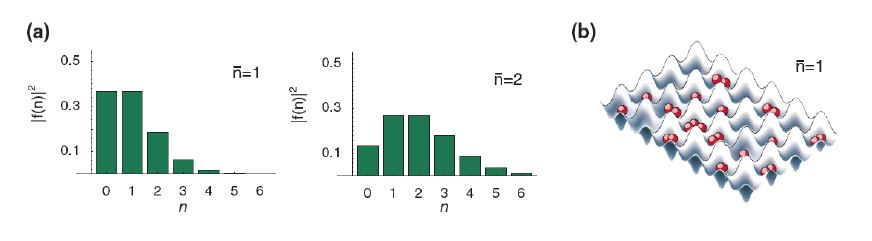
\includegraphics[width=0.8\columnwidth]{Figures/f(n)_SF.JPG} 
	\caption{\textbf{(a)}The statistics for the number of particles per lattice site $n$ for a filling fraction of $\bar{n}=1$ and $\bar{n}=2$ in the superfluid phase. \textbf{(b)} Illustration of the particles in the lattice. There will be large fluctuations of the number of particles found at each lattice site at a given time. Figure and caption adopted from \cite{greiner}.}
	\label{fig:f(n)_SF} 
\end{figure}
Since bosonic operators at different sites commute, the superfluid state can be factorized into a product of local coherent states.
Coherent states are eigenstates of the annihilation operator $\hat{a} \ket{\alpha} = \alpha \ket{\alpha}$, where $|\alpha |^2$ can be considered the particle density of the system, and $\alpha = |\alpha| e^{i \phi}$, with $\phi$ being a global phase. Utilizing the coherent state form of the wavefunction (eq. \eqref{stateSF}) the average filling fraction $\bar{n}$ can be calculated
\begin{equation}
	\bar{n} = \braket{\hat{n}_i} = \bra{\Psi_{SF}} \hat{a}_{j}^{\dag} \hat{a}_{j} \ket{\Psi_{SF}} = \frac{N}{N_L} \; ,
\end{equation}
as well as the fluctuations of particle number per site
\begin{equation}
	\frac{\sqrt{\Delta \bar{n}^2}}{\bar{n}} \sim \frac{1}{\sqrt{\bar{n}}} \; .
\end{equation}
Therefore, the probability distribution for the number of atoms at a given site is Poissonian, which can be seen in figure \ref{fig:f(n)_SF}. Due to the relatively large fluctuation of particle number per site, one would find a somewhat random number of atoms at a given site in a measurement. In the presence of a finite interaction, $U$, the resulting distribution would be sub Poissonian due to number squeezing \cite{greiner}.


\subsection{Mott-Insulator Phase}
In the case of negligible tunneling, only the on-site interaction between the atoms has to be taken into account, and the Bose-Hubbard Hamiltonian reduces to
\begin{equation}
	\hat{H} = \hat{H}_U = \frac{U}{2} \sum_{i} \hat{n}_i \left( \hat{n}_i -1 \right) \; ,
	\label{hamilMott}
\end{equation}
which is quadratic in $\hat{n}_i$. This heavily penalizes having multiple particles at the same site. Thus, the ground state of the system will be an equal distribution of all the particles throughout the lattice. Any fluctuations from this average will increase the energy, whereby the phase is said to be incompressible \cite{Gemelke2009}. This incompressibility can be formulated as $\frac{\partial n}{\partial \mu} = 0$, where $\mu$ is the chemical potential, and is the defining property of the Mott-Insulator \cite{manybodyBloch}.\\
\begin{figure}[!h]
\centering
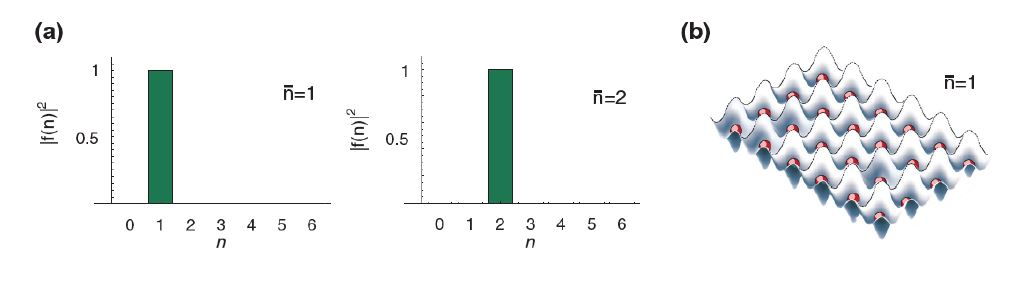
\includegraphics[width=0.8\columnwidth]{Figures/f(n)_M.JPG} 
\caption{\textbf{(a)}The statistics for the number of particles per lattice site $n$ in the Mott-insulator phase, for a filling fraction of $\bar{n}=1$ and $\bar{n}=2$. \textbf{(b)} Illustration of the particles in the lattice. The particles does not hop around in the lattice and are equally distributed. Caption and figure are adapted from \cite{greiner}.}
\label{fig:f(n)_M} 
\end{figure}
Consider the case $\bar{n} = 1$, (average filling of one particle per site). This can be described by a state with a single particle located on each site \cite{manybodyBloch}
\begin{equation}
	\ket{\Psi_{Mott}} = \prod_j \hat{a}_{j}^{\dag} \ket{0} \; .
	\label{eq:MIstate}
\end{equation}
This is a simple product of local Fock states with precisely
one atom per site, which is illustrated in figure \ref{fig:f(n)_M}. This is the configuration of atoms, which minimizes the energy with regards to the Hamiltonian of eq. \eqref{hamilMott}. Any fluctuation from unit occupancy will increase the energy, as merely a single double occupancy will increase the energy by $U$. Thereby, unlike the energy spectrum of the Superfluid, the Mott-Insulator spectrum is gapped. As long as the gain in kinetic energy due to hopping, $J$, is smaller than the on-site interaction, $U$, the atoms remain localized. However, for $J > 0$ the ground state is no longer a the simple product state described in eq. \eqref{eq:MIstate} \cite{manybodyBloch}. As $J$ increases, the gap in the excitation spectrum will gradually decrease until the transition to the superfluid is reached and the spectrum becomes gapless.\\
While the Mott-Insulator phase has complete localization, the phases on the individual sites have obtained maximum uncertainty. Therefore, no phase coherence between different sites is present \cite{greiner}.


\section{Phase Transition}
Consider once again the full Bose-Hubbard Hamiltonian \eqref{BHhamil}. The superfluid and the Mott-Insulator account for the two limits of the ratio $J/U$, however, it order to understand the full phase diagram of the Bose-Hubbard model one has to derive the $U_{crit}$ for which the phase transition occurs. There are several ways of doing this - one of them is looking at a mean-field solution of the Bose-Hubbard model. For simplicity the scenario $T=0$ is treated here. Even without a change of temperature the phase transition still happens, hence the label \textit{quantum phase transition} referring to the fact that the phase transition can happen without change of external parameters \cite{Sachdev2007QPT}.\\
Applying the mean field approximation to the annihilation operator yields
\begin{equation}
	\hat{a}_j = \psi + \delta \hat{a}_j \; ,
\end{equation}
where $\psi$ is the locally constant mean field, and $\delta \hat{a}_j$ is the fluctuation term. Inserting this into the Hamiltonian yields
\begin{equation}
	\hat{H}_{MF} = -J \sum_{\langle i,j \rangle} \left( \psi^* + \delta \hat{a}_{i}^{\dag} \right) \left( \psi + \delta \hat{a}_{j} \right) + \text{int.}
\end{equation}
Instead of considering the Hamiltonian as a whole, it can be considered as a sum of local on-site Hamiltonians
\begin{equation}
	\hat{H}_{MF} = \sum_{i} \hat{h}_i \; .
\end{equation}
For a homogeneous system $\hat{h}_i = \hat{h}_j \; \; \forall i,j$. One can write the kinetic part of the Hamiltonian locally if one assumes small fluctuations from the mean field
\begin{align}
  \hat{a}_{i}^{\dag} \hat{a}_{j} &= \left( \psi^* + \delta \hat{a}_{i}^{\dag} \right) \left( \psi + \delta \hat{a}_{j} \right) \nonumber \\
  &= \psi^* \psi + \psi^* \delta \hat{a}_j + \psi \delta \hat{a}_{i}^{\dag} + \delta \hat{a}_{i}^{\dag} \delta \hat{a}_{j} \nonumber \\
  & \approx \psi^* \psi + \psi^* \left( \hat{a}_j - \psi \right) + \psi \left( \hat{a}_{i}^{\dag} - \psi^* \right) \nonumber \\
&= \psi^* \hat{a}_j + \psi \hat{a}_{i}^{\dag} - \psi^* \psi
\end{align}
Since every term only contains a single index, one can let $j \rightarrow i$ leaving a local description
\begin{equation}
	\hat{h}_i = J z \psi^* \psi - J z \left( \psi^* \hat{a}_i + \psi \hat{a}_{i}^{\dag} \right) + \frac{U}{2} \hat{n}_i \left( \hat{n}_i -1 \right) + \mu_i \hat{n}_i \; ,
	\label{localhamil}
\end{equation}
where $z$ is the number of neighbours of site $i$ \cite{vanoosten}. The last term added is a chemical potential, which is needed due to the lack of a fixed particle number locally prompting the use of a Grand Canonical Ensemble description.\\
Landau theory is a general theory regarding phase transitions, which states that in the vicinity of a critical point, one may expand the free energy in a power series of some order parameter $m$. Thus, in order to find $U_{crit}$, equation \eqref{localhamil} must be minimized. In this case this order parameter is the mean field, hence
\begin{equation}
	E_{MF} = \text{const. } + a |\psi|^2 + b |\psi|^4 + \ldots \label{eq:landau}
\end{equation} 
Plotting this yields an effective potential, seen in figure \ref{fig:landau}, which dictates certain properties of the system.
\begin{figure}[!h]
\centering
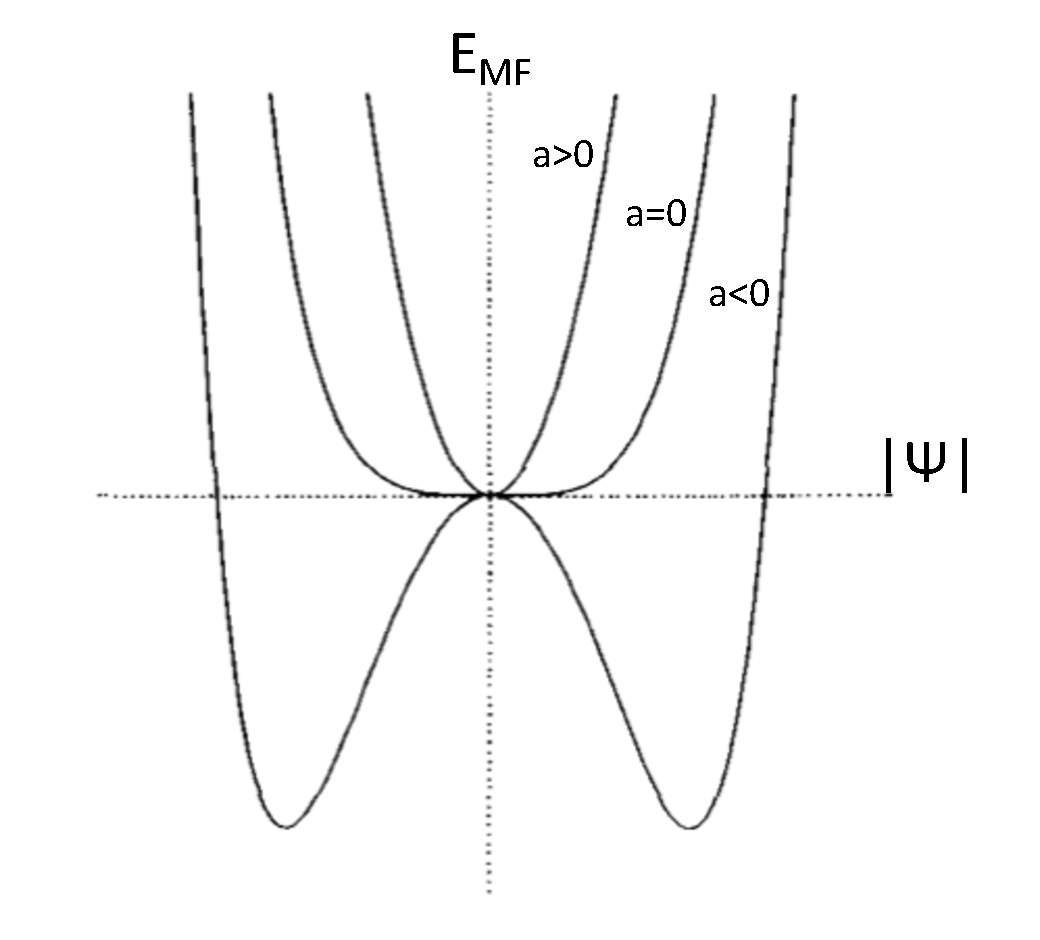
\includegraphics[width=0.7\columnwidth]{Figures/Landau_theory.pdf} 
\caption{	\textit{Effective potential as function of the order parameter $\psi$. For $a<0$ the properties of the potential change from having a single, central minimum to having two separated minima. This is an example of spontaneous symmetry breaking associated with a phase transition. \cite{plischke}}}
\label{fig:landau} 
\end{figure} 

The potential is symmetric in the complex plane allowing the system to have any phase. Furthermore, at some critical value of $a$, (here $a = 0$), the potential will shift from having a single central minimum to having minima at some $|\psi|$. This is a U(1) spontaneous symmetry breaking, which in Landau theory is associated with a phase transition \cite{plischke}. Thus, one need to compute the parameter $a$ of equation \eqref{eq:landau}.\\
One method is using second order perturbation theory, where the $\hat{\psi} = 0$ case is solved exactly, followed by adding a small $\hat{\psi}$ as a perturbation
\begin{equation}
	\hat{h}_{i}^{(0)} = J z \left( \psi^* \psi \right) + \frac{U}{2} \hat{n}_i \left( \hat{n}_i -1 \right) - \mu \hat{n}_i \; .
\end{equation} 
Since the zero-order solution only contain number operators, the ground state of the solution can be expressed in the Fock basis:
\begin{align*}
	\ket{0} \quad &\text{for} \quad \mu < 0 \\
	\ket{1} \quad &\text{for} \quad 0 \leq \mu < U \\
	\ket{2} \quad &\text{for} \quad U \leq \mu < 2 U \\
	& \vdots
\end{align*} 
Adding on the first order perturbation to the energy
\begin{equation}
	E_{i}^{(1)} = \bra{n} \delta \hat{a}_i \ket{n} = 0 \; ,
\end{equation}
yields nothing, thus requiring the use of a second order perturbation
\begin{equation}
	E_{i}^{(2)} = \sum_{n \neq g} \frac{|\bra{n} \delta \hat{h}_i \ket{g}|^2}{E_{g}^{(0)} - E_{n}^{(0)}} \; .
\end{equation}
Here the perturbation Hamiltonian
\begin{equation}
	\hat{h}_i = - z J \left( \hat{a}_i \psi^* + \psi \hat{a}_{i}^{\dag} \right)
\end{equation}
contains only single creation/annihilation operators, whereby
\begin{equation}
	\bra{n} \delta \hat{h}_i \ket{g} = 0 \quad \text{for} \quad |n - g| \neq 1 \; .
\end{equation}
Hence, for each annihilation and creation operator only two matrix elements will give a contribution
\begin{align*}
	\bra{n}  \hat{a}_{i}^{\dag} \ket{n-1} &= \sqrt{n} \braket{n|n} \\
	\bra{n+1}  \hat{a}_{i}^{\dag} \ket{n} &= \sqrt{n+1} \braket{n|n} \\
	& \vdots
\end{align*}
With this the second order perturbation energy reduces to
\begin{align}
	E_{i}^{(2)} &= \left( J z \right)^2 |\psi|^2 \left( \frac{n}{E_{g}^{(0)}- E_{n-1}^{(0)}} +  \frac{n+1}{E_{n}^{(0)}- E_{n+1}^{(0)}} \right) \nonumber \\
	&= \left( J z \right)^2 |\psi|^2 \left( \frac{n}{U(n-1) - \mu} + \frac{n+1}{\mu - U n} \right) \; .
\end{align}
Since $a$ is the pre-factor of all terms proportional $|\psi|^2$, collecting those across from all the perturbations yields the approximation 
\begin{equation}
	a = J z + \left( J z \right)^2 |\psi|^2 \left( \frac{n}{U(n-1) - \mu} + \frac{n+1}{\mu - U n} \right) \; .
\end{equation} 
As stated earlier $U_{crit}$ can be found from $a = 0$:
\begin{equation}
	0 \overset{!}{=} 1 + \frac{n}{\bar{U} (n-1) - \bar{\mu}} + \frac{n+1}{\bar{\mu} - \bar{U} n} \; ,
\end{equation}
with $\bar{mu} = \frac{\mu}{J z}$ and $\bar{U} = \frac{U}{J z}$. Finally, the solution for the chemical potential is \cite{vanoosten}
\begin{equation}
	\bar{mu}_{\pm} = \frac{1}{2} \left( \bar{U}(2n -1) \pm \frac{1}{2} \sqrt{\bar{U}^2 - 2 \bar{U} (2 n +1)} \right) \; .
\end{equation}
Understanding this result can be done be examining figure \ref{fig:SFMOTT}, which displays a phase diagram of the Bose-Hubbard model.  
\begin{figure}[h]
	\centering
	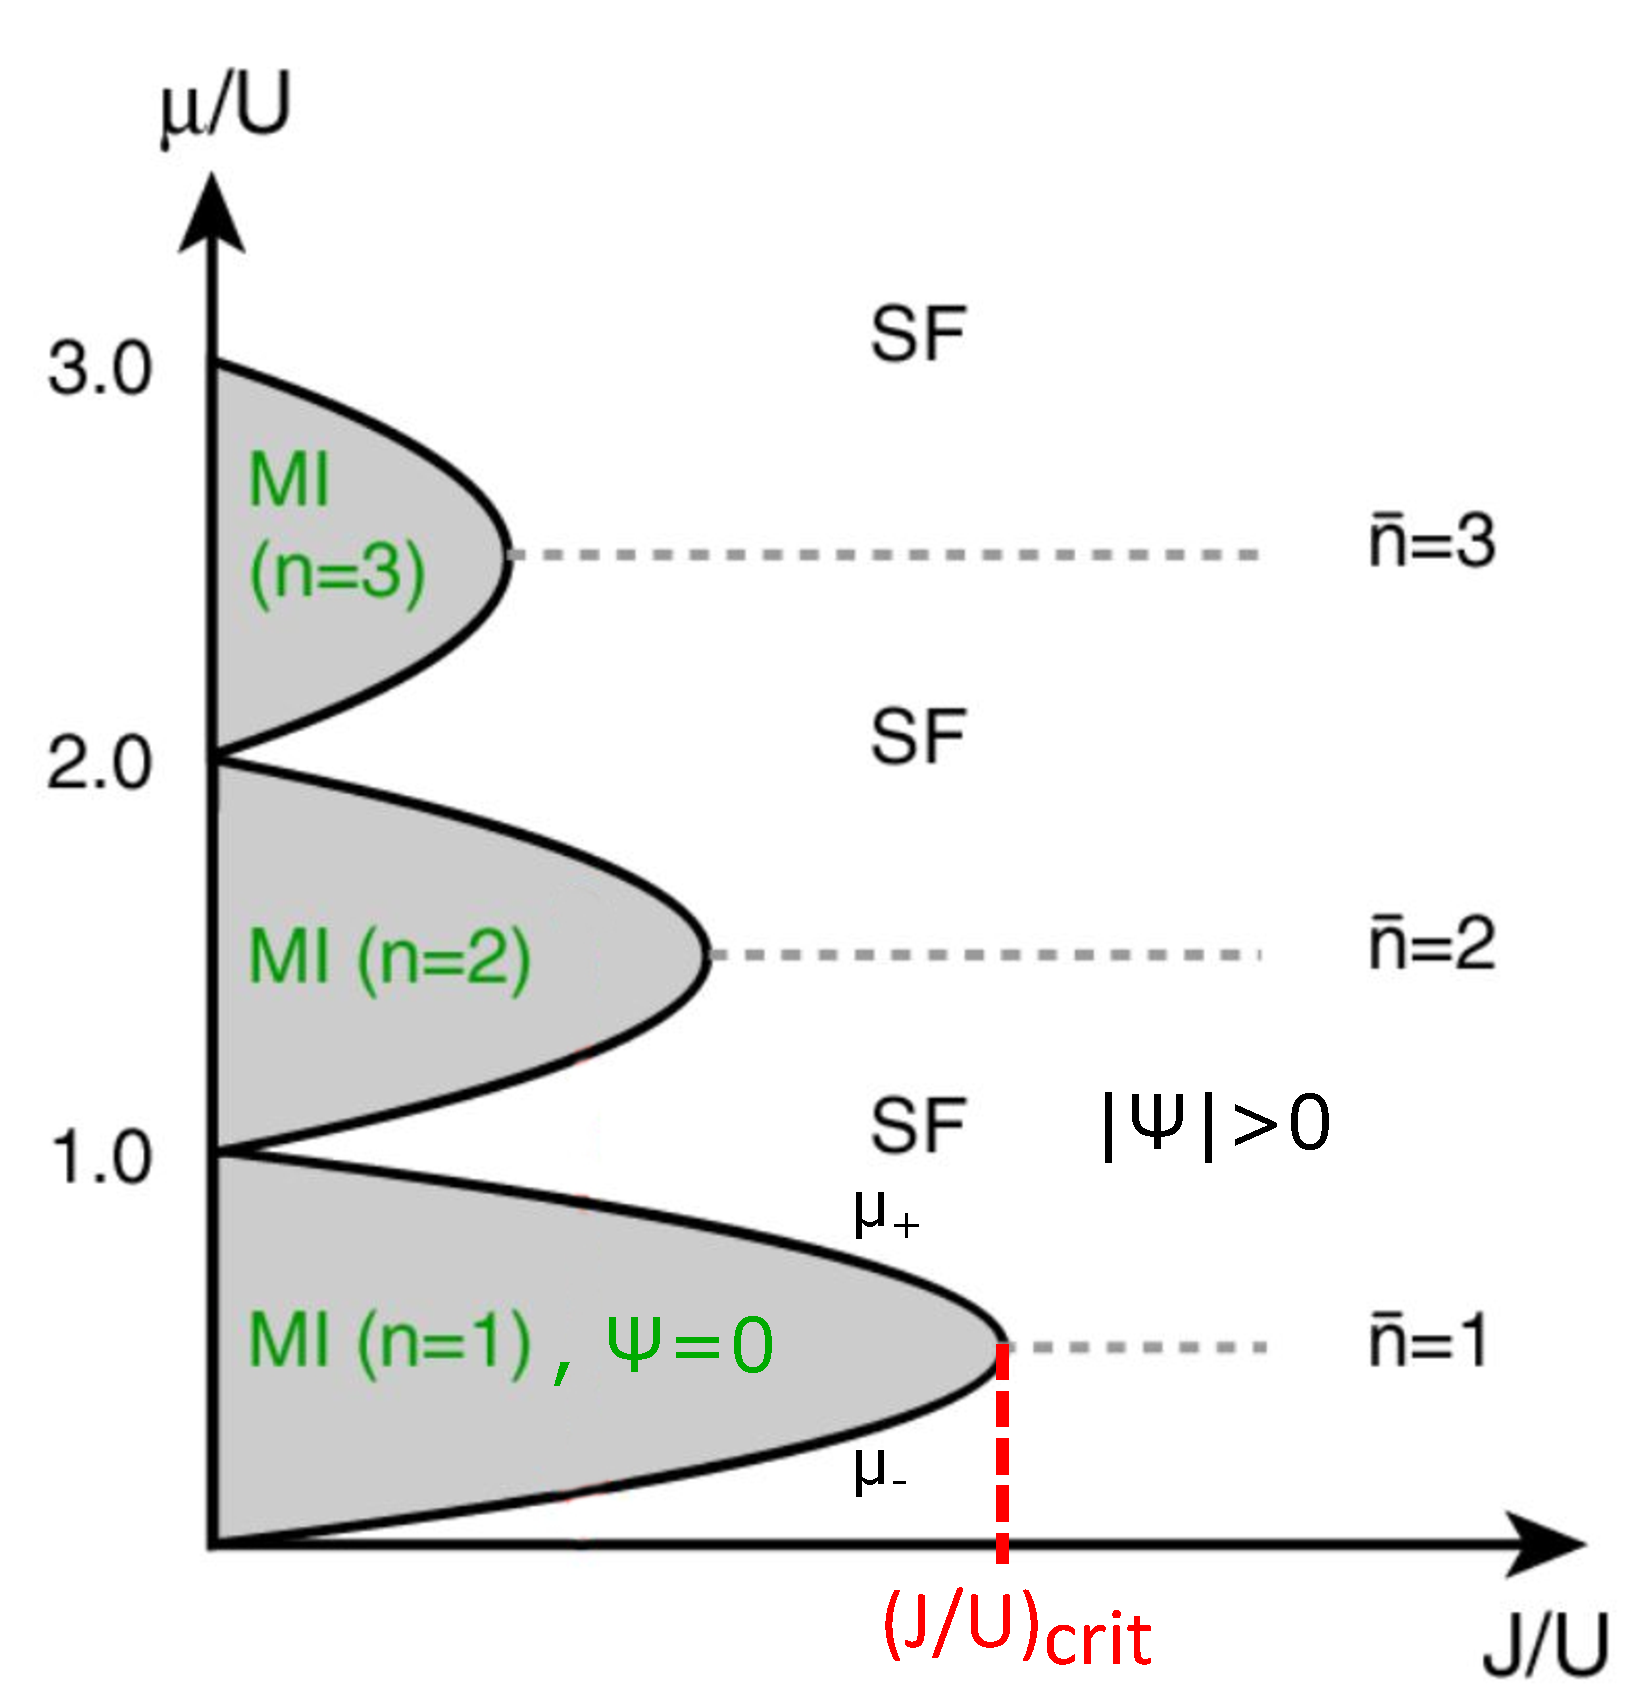
\includegraphics[width = 0.7\textwidth]{Figures/SFMottPhase.pdf}
	\label{fig:SFMOTT}
	\caption{\textit{Phase diagram of Bose-Hubbard model for T = 0. Grey areas mark the Mott Insulator phase for different number of particles per site, while white regions mark the superfluid phase. \cite{greiner}}}
\end{figure}
The $\mu_{\pm}$ curves encloses the region where the system is in the Mott Insulating phase. $(1/\bar{U})_{crit} = (J/U)_{crit}$ can be read off the graph from the point, where the two curves $\mu_{\pm}$ meet. As mentioned earlier, no fluctuations take place in the Mott Insulator, whereby the particle number per site is well defined, while it for the superfluid can take many values. As the chemical potential increases each site can accommodate more particles as long as the increase in chemical potential compensates the increased energy due to interactions between the particles.\\
The mean-field solution of the Bose-Hubbard model is only an approximation, which proves quite inaccurate for one dimension. This is seen when comparing the critical ratio for the mean-field approach, $\left( U/J \right)_{crit}^{MF,1D} = 11.66$, with numerical results computed using the DMRG method, $\left( U/J \right)_{crit}^{DMRG,1D} = 3.37$, \cite{Kuhner2000}. Nevertheless, it gives a good intuitive feeling of the physics taking place and how one can describe them without resorting to diagonalizing the Hamiltonian.\\